\documentclass[11pt,a4paper]{article}
\usepackage[margin=2.2cm]{geometry}
\usepackage{graphicx,booktabs,amsmath,siunitx,hyperref,caption,float,xcolor}
\usepackage[numbers,sort&compress]{natbib}
\captionsetup{font=small,labelfont=bf}
\sisetup{detect-all}
\hypersetup{colorlinks=true,linkcolor=blue!50!black,citecolor=blue!50!black,urlcolor=blue!50!black}
\title{\textbf{LATCH: a load-sequence-sensing, any-angle stance-control knee joint for knee--ankle--foot orthoses, designed and validated on 9{,}781 real strides}}
\author{Design package and analysis report}
\date{October 2026}
\begin{document}
\maketitle

\begin{abstract}
\noindent People with quadriceps paralysis (polio survivors, incomplete spinal-cord injury, stroke) usually walk in knee--ankle--foot orthoses (KAFOs) whose knee is locked straight for the whole gait cycle, forcing hip hiking, circumduction and vaulting. Stance-control knee joints that free the knee in swing cost US\$1{,}700--3{,}500 per joint and the only purely mechanical ones either need a cable from the ankle or a gravity pendulum that locks only at full extension. We asked whether a knee joint can decide stance from swing using \emph{only the loads it already carries}. Using a public multi-speed walking dataset (51 subjects, 381 treadmill trials, 0.34--2.23\,m/s) we first showed that any pendulum trigger mounted on the thigh is corrupted by the knee's own accelerations (up to 14\,m/s$^2$ at toe-off), so that no pendulum length, mount height or damping achieved both reliable locking at heel strike and release before swing. We then designed a joint in which a fine-pitch ratchet (3.75$^\circ$ resolution, locks at any knee angle) is engaged and released by the \emph{sign sequence of the external knee moment}: a flexion load on the pawls sets a mechanical latch, a subsequent extension load on a sprung hyperextension stop releases the pawls, a friction drag ring on the knee axle keeps them lifted while the knee flexes in swing and drops them during swing extension, and two rotary dampers and a dashpot provide the required 0.1--0.3\,s time constants. Simulated on 9{,}781 valid strides with a causal state machine driven by measured knee kinematics and inverse-dynamics moments, the design locked at heel strike in 99.2\% of strides at speeds $\le$1.5\,m/s, was unlocked while a buckling load was present in 0.27\%, falsely blocked swing flexion in 0.23\%, released before pre-swing flexion in 89.6\% and never released in 3.6\% (a safe, stiff-knee stride). The knee angle at heel strike in the dataset was $7.4\pm6.0^\circ$ (64\% of strides $>5^\circ$), which quantifies why single-notch full-extension locks fail. The complete joint is modelled parametrically (22 components, STEP and STL supplied): a laser-cut steel load path (two phased toothed clevis plates, 3-tooth hook pawls, 12\,mm pin) with 3D-printed control parts, bill of materials US\$74, plane-stress FE peak tooth stress 250--280\,MPa at the 70\,N$\cdot$m design moment and 540--600\,MPa at a 150\,N$\cdot$m proof moment (17-4PH H900 yield 1{,}170\,MPa). We give the full validation protocol for bench and gait-laboratory testing.
\end{abstract}

\section{Introduction}
\subsection{The problem}
Between 12 and 20 million people live with the paralytic consequences of poliomyelitis, and in the countries that reached full vaccination coverage only after 1988 most of them are still children or young adults \cite{gonzalez2010,groce2014}. Spinal-cord injury adds 20.6 million prevalent cases worldwide, most of them incomplete \cite{gbdsci2023}, and 40--60\% of stroke survivors show knee hyperextension in stance because they cannot control the knee \cite{cooper2012}. When the quadriceps cannot hold the knee, the standard orthotic answer is a knee--ankle--foot orthosis (KAFO) with a drop lock: the knee is held straight through the whole gait cycle. The locked knee is stable but forces an energy-inefficient long-leg gait (hip hiking, circumduction, vaulting), and long-term use is associated with hip and lumbar compensations and skin damage \cite{locked_kafo_iatrogenic2023,yakimovich2009}. Device abandonment is common across assistive technology (29\% overall \cite{phillips1993}); in a cohort of 98 polio survivors 24\% had stopped using their custom KAFO \cite{jrm2021_kafo_polio}. Globally only about one person in ten who needs prosthetic or orthotic services has access to them, and two to four times more people need orthoses than prostheses \cite{who_ispo2017,ispo_pando_day}; users in Sierra Leone and Malawi rank safety and uneven-ground walking among their main complaints \cite{magnusson2017}.

\subsection{Stance-control joints and why they are rare}
Stance-control knee--ankle--foot orthoses (SCKAFOs) lock the knee only while the leg bears weight and free it in swing. They normalise kinematics reliably even if the energy-cost benefit is modest \cite{davis2010,zissimopoulos2007,irby2005,yakimovich2009}. Commercial joints fall into three families. (i) Cable-released joints (Ottobock FreeWalk, Becker UTX/Stride family) unlock when the ankle dorsiflexes in late stance and lock only when the knee reaches full extension \cite{yakimovich2009}; (ii) the Fillauer Swing Phase Lock (SPL2) uses an internal gravity pendulum that drops a pawl into a single notch at full extension when the thigh is inclined forward \cite{spl2_manual}; (iii) sensor-based electromechanical and microprocessor joints (E-MAG, NEURO TRONIC, C-Brace) that cost from \euro10{,}000 to US\$37{,}000 as finished orthoses and still show 10--14\% unlock failures per step under challenging conditions \cite{neurotronic2023,schmalz2016,price_cbrace_sps}. Bare mechanical joint systems list at about US\$1{,}700 (FreeWalk kit) to \pounds3{,}500 (SPL2) \cite{price_freewalk_kit,price_spl2_uk}. The recurring engineering limitation identified by Yakimovich et al.\ is ``dependence on specific joint angles to switch between stance and swing modes'' \cite{yakimovich2009}: a user who falls short of full extension in terminal swing is left unsupported \cite{resna2019_eveleight}. Becker markets the SafetyStride specifically as resisting flexion at any angle \cite{becker_safetystride}; research joints with any-angle capability have used hydraulics (69\,N$\cdot$m \cite{yakimovich2006}), a linear piston resisting $>150$\,N$\cdot$m \cite{lemaire2009}, a quasi-passive spring clutch \cite{shamaei2014}, a three-tooth 10$^\circ$-pitch ratchet \cite{resna2019_eveleight}, and most recently a low-cost solenoid-driven serrated ring \cite{embc2025solenoid}. None of these is simultaneously any-angle, electronics-free, cable-free, pendulum-free and open.

\subsection{Contribution}
This report presents LATCH (Load-Actuated, Thigh-Cable-free, any-angle stance-Control Hinge), a KAFO knee joint that decides stance from swing using only the external knee moment it already carries, with no pendulum, cable, battery or sensor. Three things are new. First, a data-driven negative result that motivates the design: driven by the measured kinematics of 51 subjects, a thigh-mounted pendulum cannot be made reliable at any length, mount height or damping (Section~\ref{sec:pendulum}). Second, a load-sequence stance detector that is realisable with two springs, a friction ring, two rotary dampers and a dashpot, and whose per-stride performance we quantify on 9{,}781 strides across eight speeds (Section~\ref{sec:logic}). Third, a complete parametric design package (CAD, finite-element sizing, bill of materials, assembly and validation protocol) that uses laser-cut steel for the load path and 3D printing for the control mechanism, at a parts cost of US\$74 (Sections~\ref{sec:design}--\ref{sec:structural}).

\section{Methods}
\subsection{Gait data}
We used the Fukuchi et al.\ public walking dataset \cite{fukuchi2018} (``WBDS''; figshare 10.6084/m9.figshare.5722711, v3 release containing 51 adult subjects), restricted to its treadmill trials: eight speeds per subject (40--145\% of comfortable speed), 30\,s each, giving 381 trials with 150\,Hz marker trajectories, 300\,Hz split-belt force plates and gait-cycle-normalised joint moments from inverse dynamics. From the markers we computed, for the right leg, the thigh inclination from vertical $\theta$ (greater trochanter to lateral knee marker), the knee flexion angle (thigh versus shank segments), and the position and acceleration of points on the lateral thigh upright 0--20\,cm above the knee axis, after 8\,Hz low-pass filtering. Right heel strikes and toe-offs were detected as force-plate contacts validated by the centre of pressure lying within 18\,cm of the right heel and ankle markers. Strides with implausible stance fraction ($<50\%$ or $>72\%$ of the cycle) or duration (outside 0.6--2.4\,s) were excluded, leaving 9{,}781 strides from 51 subjects at 0.34--2.23\,m/s (mean body mass 67.8\,kg). The knee moment curve of each trial (N$\cdot$m/kg; positive = internal extensor = external flexion load) was mapped onto each stride by percentage of cycle.

\subsection{Mechanism simulation}
Both trigger concepts were simulated as causal state machines sampled at 150\,Hz and driven by the measured kinematics and moments. Because the dataset comes from unimpaired walkers whose knees flex 15--20$^\circ$ during loading response, we applied a \emph{virtual lock}: while the pawls are engaged the knee angle presented to the mechanism cannot exceed the angle at engagement (the ratchet permits extension only), which is what the orthosis would enforce. Pawls carrying an external flexion load cannot be lifted (self-holding tooth geometry); they can only be released when that load is zero.

\paragraph{Pendulum trigger.} A physical pendulum of effective length $L_\mathrm{eff}$ and damping ratio $\zeta$ pivots on the thigh upright at height $s$ above the knee axis and reads its angle $\psi$ relative to the upright: $\ddot\psi = -(g/L_\mathrm{eff})\,[(1+a_y/g)\sin\phi + (a_x/g)\cos\phi] - 2\zeta\omega_n\dot\psi - \ddot\theta$, $\phi=\psi+\theta$, with $(a_x,a_y)$ the measured pivot acceleration and $\pm35^\circ$ travel stops. A bistable toggle arms the lock when $\psi\le-\theta_L$ and disarms it when $\psi\ge+\theta_U$. We swept $L_\mathrm{eff}\in[3,40]$\,cm, $s\in\{0,10,20\}$\,cm and $\zeta\in\{0.3,0.7,1.5,3\}$ with $\theta_L=\theta_U=5^\circ$.

\paragraph{Load-sequence trigger (LATCH).} The joint has three mechanical inputs: the external flexion moment carried by the engaged pawls; the external extension moment carried by a sprung hyperextension stop with 1\,mm of travel before a hard stop; and the direction of knee rotation sensed by a friction-drag ring on the knee axle with a dead band $\delta$. The logic (Fig.~\ref{fig:timeline}) is: (1) a pawl load above $M_\mathrm{pawl}$ sets a LATCH that decays $T_\mathrm{latch}$ after the pawl unloads (rotary damper); (2) a stop load above $M_\mathrm{thr}$ while LATCH is set, or sustained for longer than $T_\mathrm{long}$ (dashpot timer), lifts the pawls and keeps them lifted while the stop remains loaded; (3) the drag ring holds the pawls lifted while the knee flexes and lets them drop, after a delay $t_\mathrm{drop}$ set by a second rotary damper, once the knee has extended by $\delta$; (4) the ratchet teeth cover knee angles $-5^\circ$ to $30^\circ$, so pawls dropped at larger flexion ride a smooth rim and engage on reaching the toothed sector. Thresholds are per kilogram of body mass and are set on the device by spring preload screws. The design point is $M_\mathrm{thr}=0.05$, $M_\mathrm{pawl}=0.08$\,N$\cdot$m/kg, $T_\mathrm{latch}=0.15$\,s, $T_\mathrm{long}=0.30$\,s, $\delta=15^\circ$, $t_\mathrm{drop}=0.10$\,s, $t_\mathrm{lift}=0.03$\,s.

\paragraph{Outcome measures (per stride).} \emph{Locked at heel strike}: pawls engaged at the next heel strike and 20\,ms later. \emph{Buckling exposure}: any instant before the pre-swing flexion onset at which the knee is unlocked while the external flexion moment exceeds 0.05\,N$\cdot$m/kg. \emph{False lock}: pawls engaged while the knee is flexing in swing. \emph{Released in time}: pawls released before the knee needs to flex 5$^\circ$ beyond its mid-stance minimum. \emph{Stiff stride}: no release before toe-off (safe failure). We also report the release instant and the ratcheting travel (clicks) per stride.

\subsection{CAD, structural sizing and finite elements}
The joint was modelled parametrically in CadQuery (OCCT kernel); every dimension in this report is a named parameter in \texttt{cad\_knee.py}, and STEP and per-part STL files are exported from the same script. Plane-stress linear elasticity (scikit-fem, quadratic triangles, gmsh meshes refined to 0.15\,mm at the loaded teeth) was used for the toothed shank plate: the external flexion moment $M$ was applied as tractions on the three engaged tooth flanks shared 50/30/20\% (a conservative allowance for pitch tolerance), with the plate fixed at its bushing seat. Pins, bushings and uprights were sized analytically.

\section{Results}
\subsection{Why a single-notch lock fails and why a pendulum cannot fix it}\label{sec:pendulum}
Knee flexion at heel strike across the 9{,}781 strides was $7.4\pm6.0^\circ$ (5th--95th percentile $-0.7$ to $18.1^\circ$); 64\% of strides exceeded 5$^\circ$ and 28\% exceeded 10$^\circ$ (Fig.~\ref{fig:rationale}A). A lock with a single notch at full extension therefore depends on the orthotist's alignment and on the user reaching that one angle every step; an any-angle lock removes the dependence.

A gravity pendulum reads the direction of apparent gravity $g-a$, not of $g$. Fig.~\ref{fig:rationale}B shows, for one subject at 1.24\,m/s, that the forward acceleration of the knee at toe-off (peaks of 9--14\,m/s$^2$ at the knee, 5--7\,m/s$^2$ 20\,cm up the thigh) tilts apparent gravity by 40--55$^\circ$ and its deceleration in terminal swing by 20--40$^\circ$, in each case in the direction that mimics the opposite gait phase. Across the full sweep (Fig.~\ref{fig:rationale}C and \texttt{sweep1.csv}) the best pendulum for locking (8\,cm, 20\,cm mount, $\zeta=3$) locked at heel strike in 99.7\% of strides but released before swing in only 2.5\%; the best for releasing (3\,cm at the knee, $\zeta=0.3$) released in 84\% but engaged the ratchet during swing flexion in 53\% of strides. Long pendulums ($L_\mathrm{eff}\ge$ 20\,cm) remove the thigh-rotation component but sit near resonance with the stride-frequency hip acceleration and miss the 130\,ms release window. Slow, heavily damped pendulums are safe but functionally equivalent to a locked knee. This is the mechanism behind the alignment sensitivity reported for pendulum joints \cite{spl2_manual,yakimovich2009}, and it is a property of inertial sensing at the knee rather than of any particular product.

\begin{figure}[H]\centering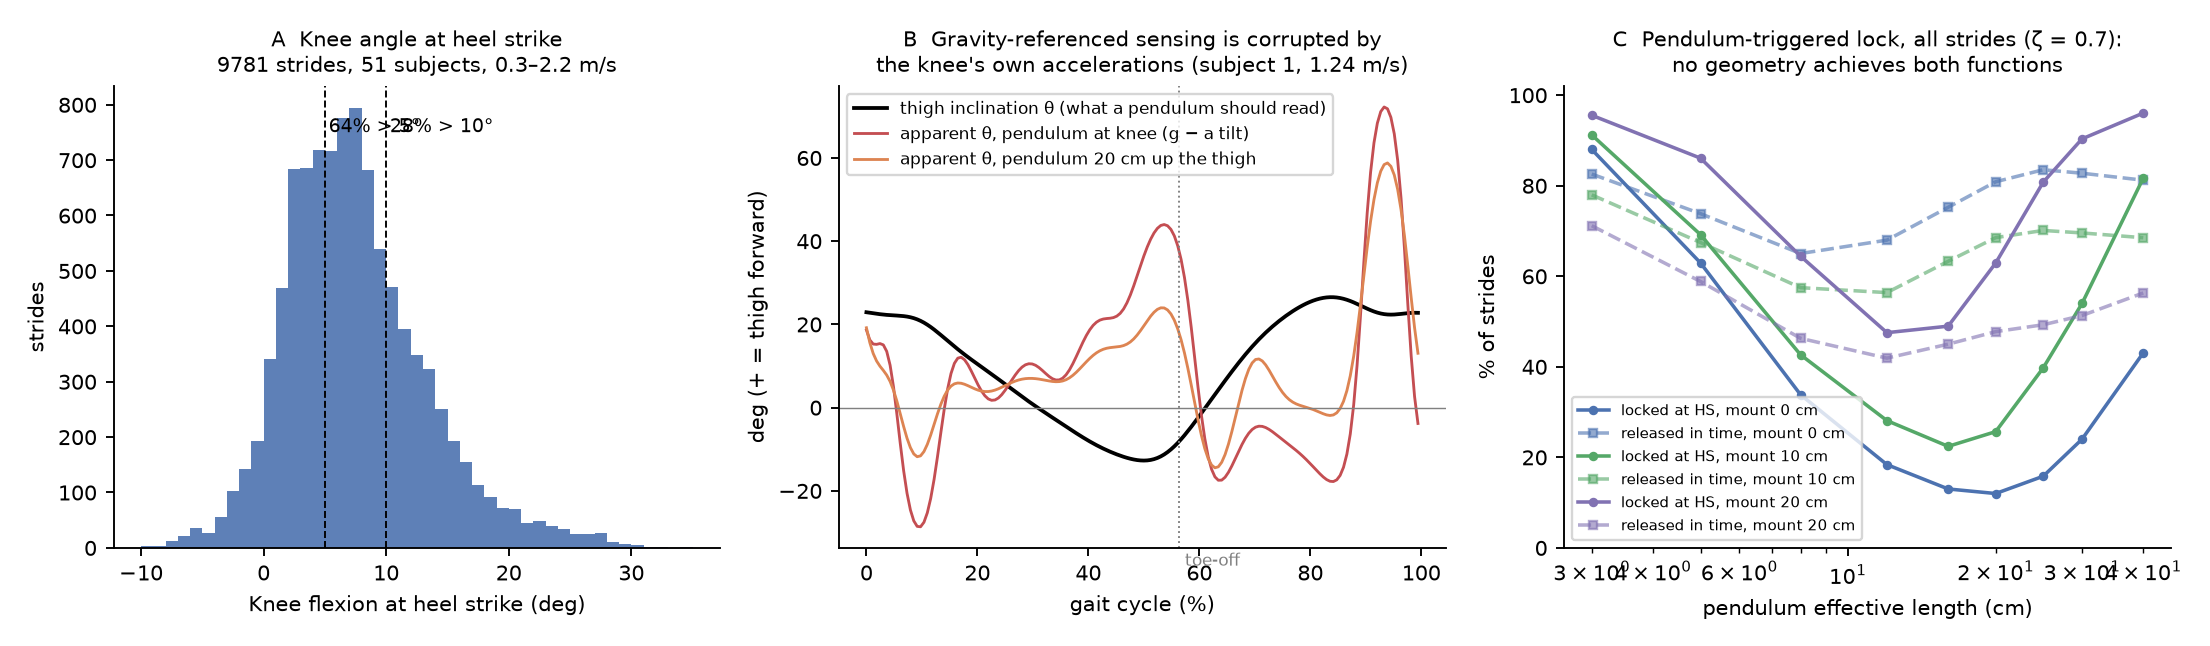
\includegraphics[width=\textwidth]{figures/fig_rationale.png}
\caption{\textbf{Data-driven rationale.} (A) Knee flexion at heel strike, 9{,}781 strides. (B) Thigh inclination and the inclination a pendulum would read (apparent gravity $g-a$) for a stride at 1.24\,m/s; the toe-off acceleration mimics ``thigh forward'' (lock) exactly when release is required, the terminal-swing deceleration mimics ``thigh back'' (release) exactly when locking is required. (C) Pendulum sweep ($\zeta=0.7$): fraction of strides locked at heel strike (solid) and released before pre-swing flexion (dashed) versus effective length for three mount heights.}
\label{fig:rationale}\end{figure}

\subsection{The load-sequence stance detector}\label{sec:logic}
Fig.~\ref{fig:timeline} shows the LATCH logic on a measured stride at 1.03\,m/s. The pawls are engaged at heel strike. The initial-contact extension moment (the ground reaction passes in front of the knee for 50--80\,ms) loads the stop but LATCH is not set, so nothing happens; during loading response the external flexion moment loads the pawls and sets LATCH; when the ground reaction moves in front of the knee at 23\% of the cycle the stop is loaded while LATCH is live and the pawls lift. The knee is now free but rests against the extension stop, which carries an extension moment of 0.3--0.65\,N$\cdot$m/kg through mid-stance: a knee under an external extension moment is self-stable, which is the biomechanical justification of releasing at this instant. At pre-swing the stop unloads and the knee flexes; the drag ring registers 15$^\circ$ of flexion within the 100\,ms pawl-drop delay and holds the pawls up through swing. At peak swing flexion the knee reverses, the ring releases the pawls after 15$^\circ$ of extension, they ride the smooth rim and ratchet over the last 20$^\circ$ (median 21.6$^\circ$ of ratcheting, about six clicks at 3.75$^\circ$ resolution) and the knee arrives at heel strike locked at whatever angle it reached.

\begin{figure}[H]\centering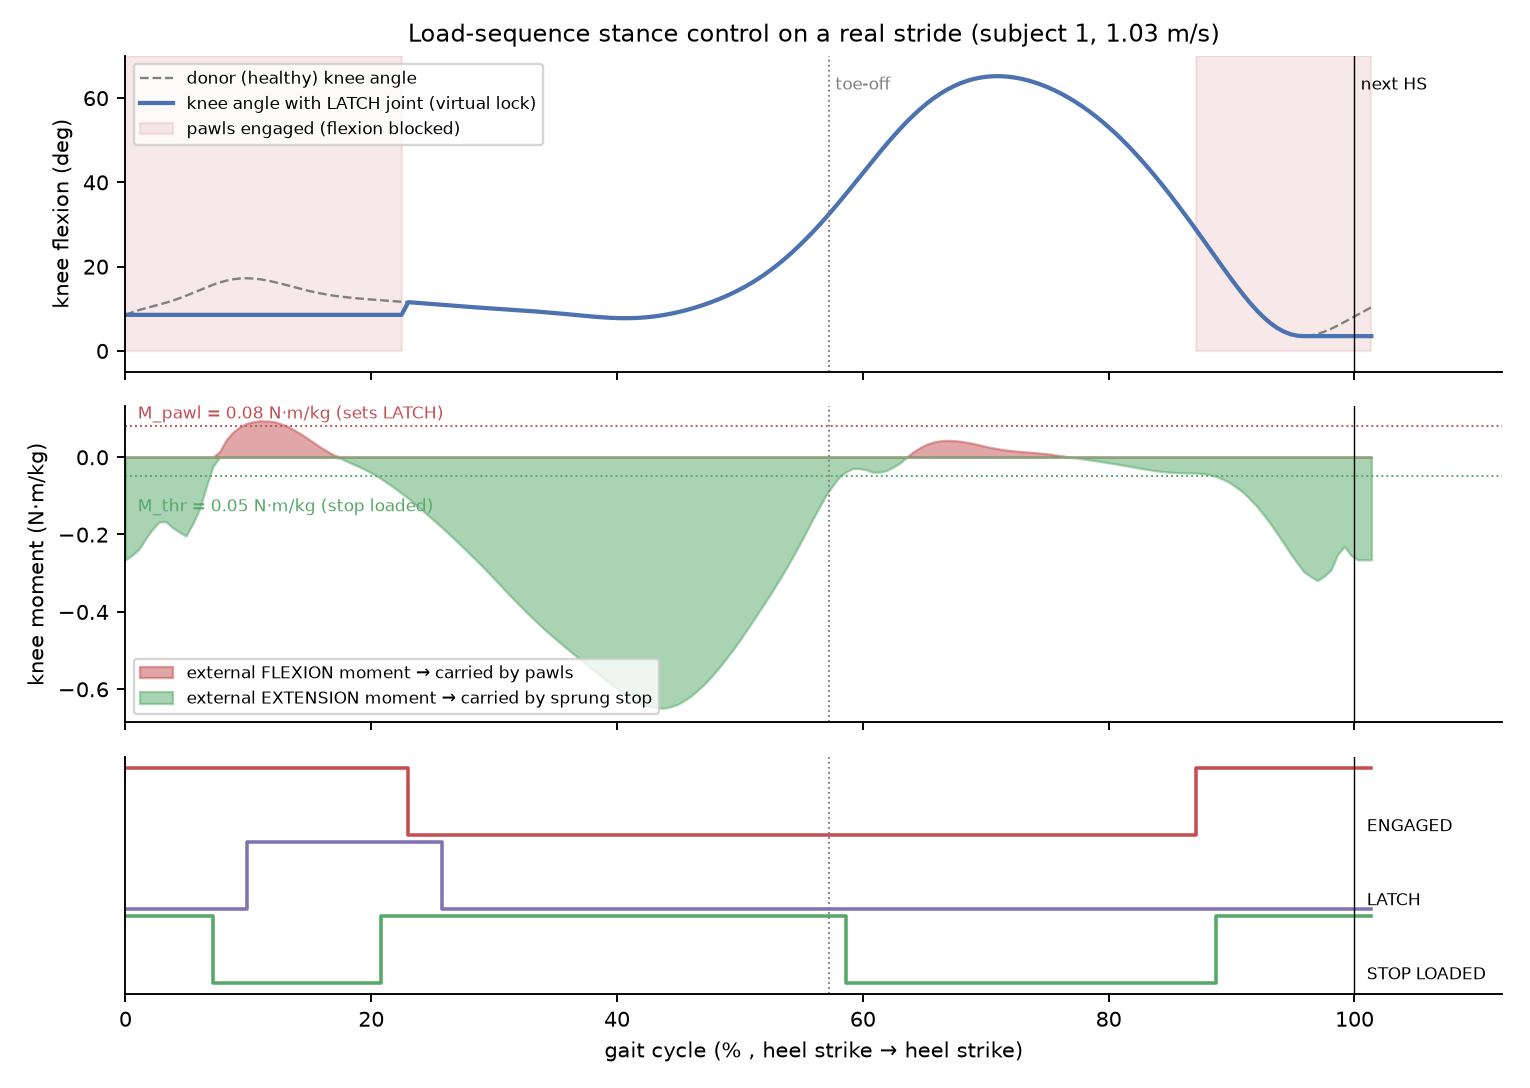
\includegraphics[width=0.92\textwidth]{figures/fig_timeline.png}
\caption{\textbf{LATCH state machine on a measured stride} (subject 1, 1.03\,m/s). Top: donor knee angle and the angle enforced by the virtual lock; shaded = pawls engaged. Middle: external knee moment; red = flexion load carried by the pawls, green = extension load carried by the sprung stop, with the two preload thresholds. Bottom: logic states.}
\label{fig:timeline}\end{figure}

Table~\ref{tab:perf} and Fig.~\ref{fig:perf} summarise performance. Within the speed range in which KAFO users walk ($\le$1.5\,m/s; 7{,}278 strides, 51 subjects) the joint was locked at heel strike in 99.2\% of strides, was exposed to a buckling load while unlocked in 0.27\%, falsely blocked swing flexion in 0.23\%, released before the knee needed to flex in 89.6\%, released late but before toe-off in a further 6.8\%, and never released (stiff-knee stride) in 3.6\%. The median release instant was 28\% of the cycle (5th--95th percentile 7--51\%). Above 1.5\,m/s performance degrades (locked at heel strike 89--93\%, exposure 7--8\%) through one specific chain: fast walkers develop a second external flexion moment in pre-swing that keeps the pawls loaded until toe-off, so LATCH is still live when the shank's deceleration loads the stop in terminal swing and the joint releases just before heel strike. A hypothetical heel-strike impact detector that allowed LATCH to be set only within 0.5\,s of heel strike would raise locking above 1.5\,m/s to 98.2\% and cut exposure to 0.9\% at no cost in the envelope (Fig.~\ref{fig:perf}C, \texttt{lock\_sensitivity.json}); we list it as the first design iteration.

\begin{table}[H]\centering\small
\caption{Per-stride performance of the design point. Envelope = speeds $\le$1.5\,m/s. ``Stiff'' strides are counted in ``not released in time''.}
\label{tab:perf}
\begin{tabular}{lccccccc}\toprule
Speed band (m/s) & $n$ & Locked at HS & Buckling exposure & False swing lock & Released in time & Stiff stride & Release (\%GC)\\\midrule
0.50 & 873 & 94.6\% & 0.0\% & 0.6\% & 93.2\% & 3.4\% & 14\\
0.69 & 1065 & 100.0\% & 0.4\% & 0.4\% & 90.6\% & 1.9\% & 20\\
0.87 & 1188 & 99.3\% & 0.0\% & 0.5\% & 86.4\% & 3.1\% & 32\\
1.06 & 1321 & 100.0\% & 0.8\% & 0.1\% & 90.2\% & 3.4\% & 28\\
1.24 & 1445 & 99.7\% & 0.3\% & 0.1\% & 87.0\% & 6.2\% & 29\\
1.43 & 1530 & 99.5\% & 0.8\% & 0.3\% & 95.6\% & 0.3\% & 28\\
1.63 & 1234 & 89.1\% & 7.7\% & 4.6\% & 92.5\% & 5.3\% & 25\\
1.79 & 1125 & 93.3\% & 6.6\% & 5.8\% & 96.8\% & 3.2\% & 26\\\midrule
Envelope $\le$1.5 & 7278 & 99.2\% & 0.27\% & 0.23\% & 89.6\% & 3.6\% & 28\\
All & 9781 & 97.2\% & 2.0\% & 1.5\% & 91.5\% & 3.4\% & 28\\\bottomrule
\end{tabular}\end{table}

\begin{figure}[H]\centering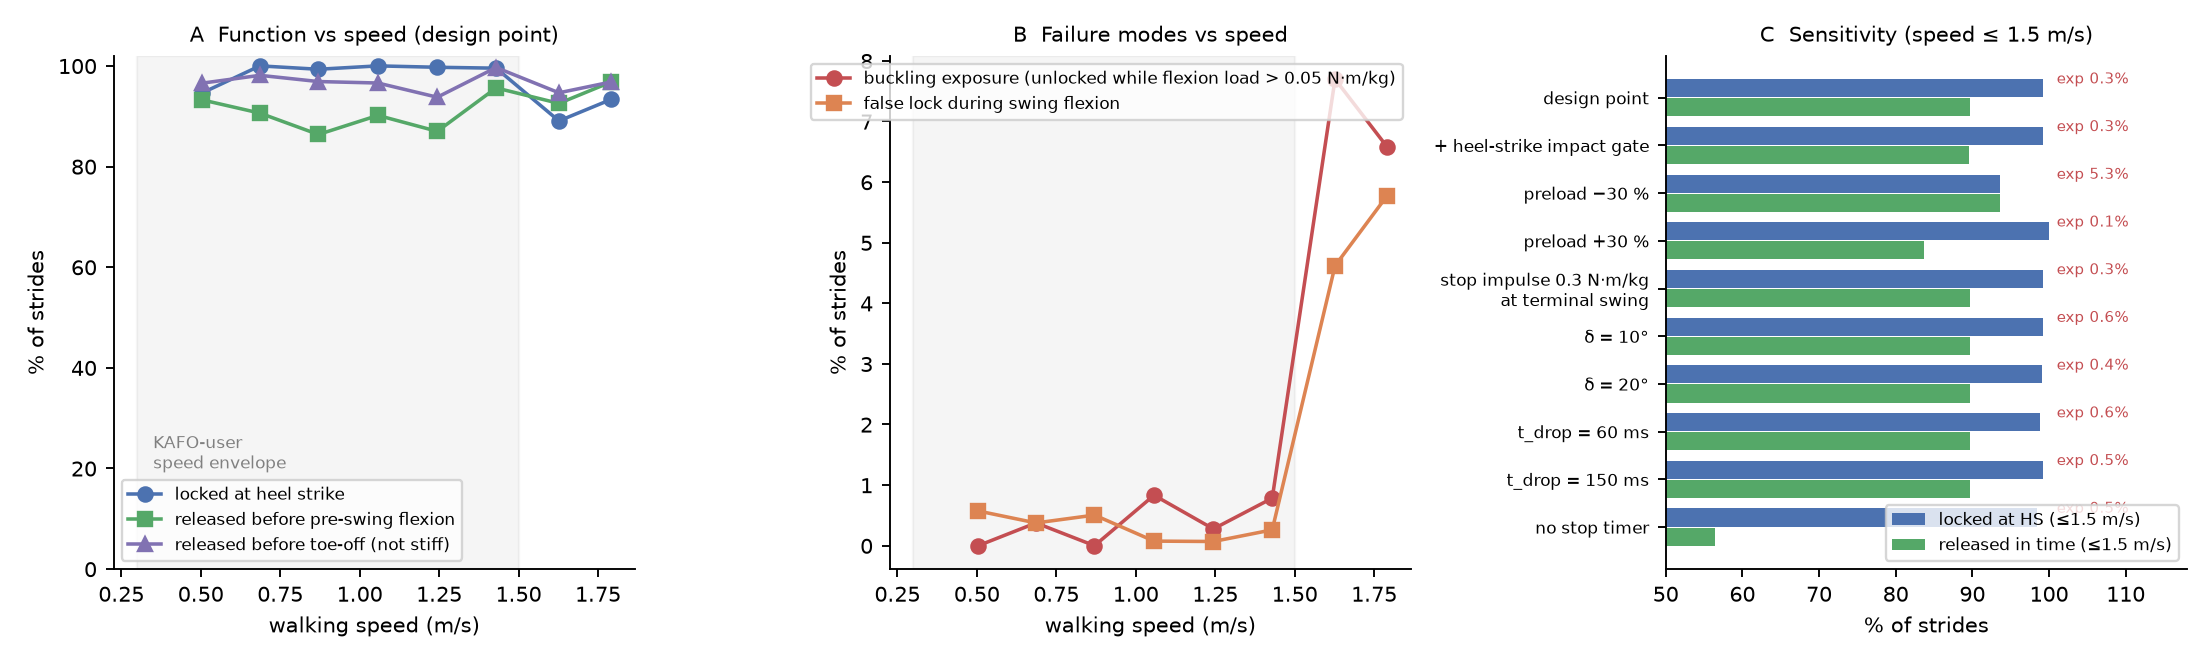
\includegraphics[width=\textwidth]{figures/fig_performance.png}
\caption{\textbf{Performance and sensitivity.} (A) Locking and release rates versus speed. (B) Failure modes versus speed; the grey band is the KAFO-user speed envelope. (C) Sensitivity of envelope performance to the heel-strike gate, preload error, a terminal-swing stop impulse, drag-ring dead band, pawl-drop delay and removal of the dashpot timer.}
\label{fig:perf}\end{figure}

The sensitivity study (Fig.~\ref{fig:perf}C) gives three design rules. (i) Preload must err high: thresholds 30\% too low reduce locking to 93.6\% and raise exposure to 5.3\%, whereas thresholds 30\% too high keep 99.99\% locking and 0.07\% exposure at the price of 7.5\% stiff strides; the preload screws should therefore be set from the user's body mass and then backed off only until swing release is observed. (ii) The dashpot timer is essential: without it, strides whose loading-response flexion moment never exceeds $M_\mathrm{pawl}$ (all slow walking, where the ground reaction stays in front of the knee) never release and 44\% of envelope strides are stiff. (iii) The drag-ring dead band and pawl-drop delay are forgiving over $\delta=10$--$20^\circ$ and $t_\mathrm{drop}=60$--150\,ms, and a 0.3\,N$\cdot$m/kg, 25\,ms stop impulse at terminal swing (shank hitting the extension stop) changes nothing because LATCH is not live at that instant. Knee moment peaks in the dataset were 0.21 (median), 0.82 (95th) and 1.06\,N$\cdot$m/kg (99th percentile) in flexion and 0.51/0.78\,N$\cdot$m/kg in extension, which fixes the structural loads below.

\section{Mechanical design}\label{sec:design}
\begin{figure}[H]\centering
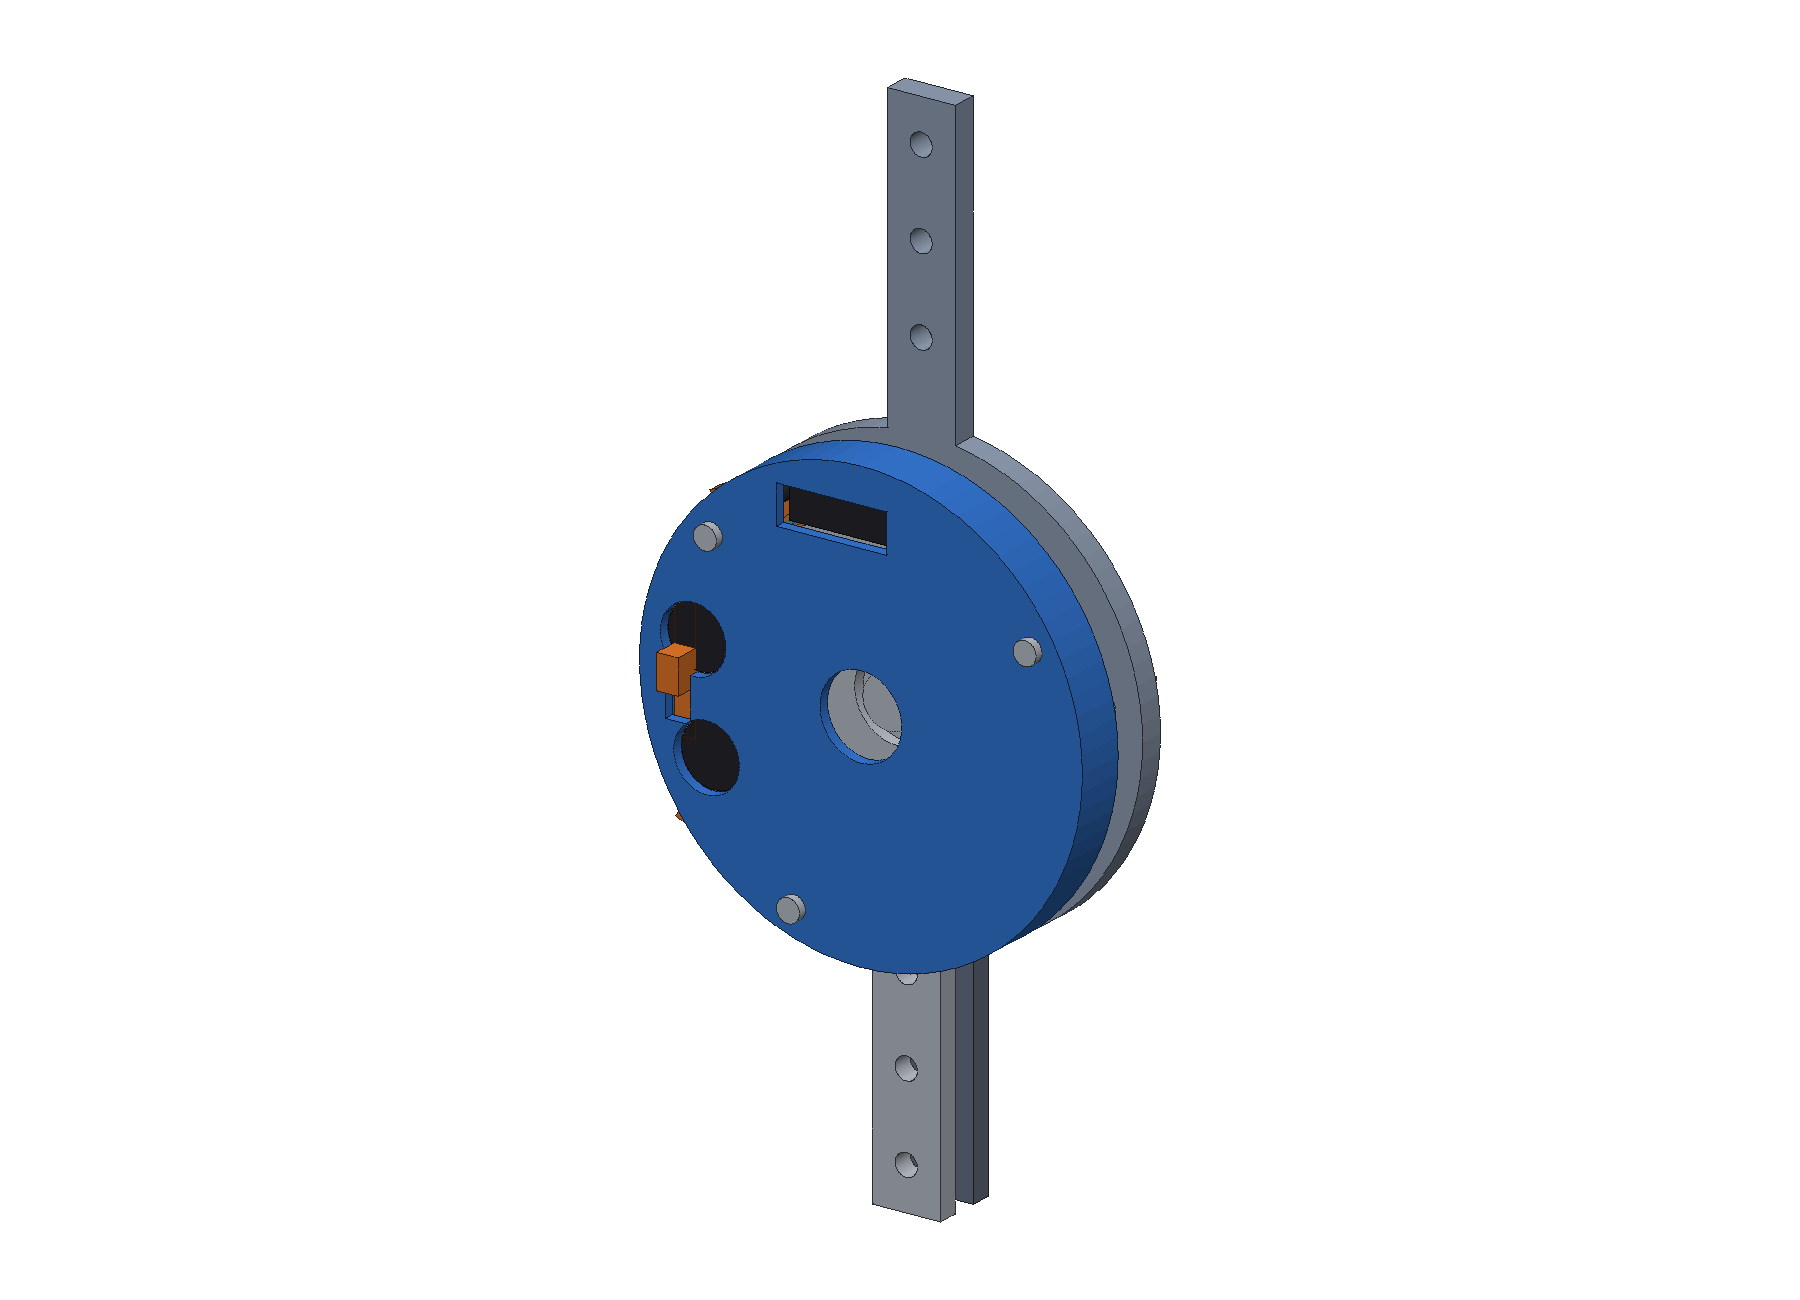
\includegraphics[width=0.48\textwidth]{figures/render_iso_closed.png}\hfill
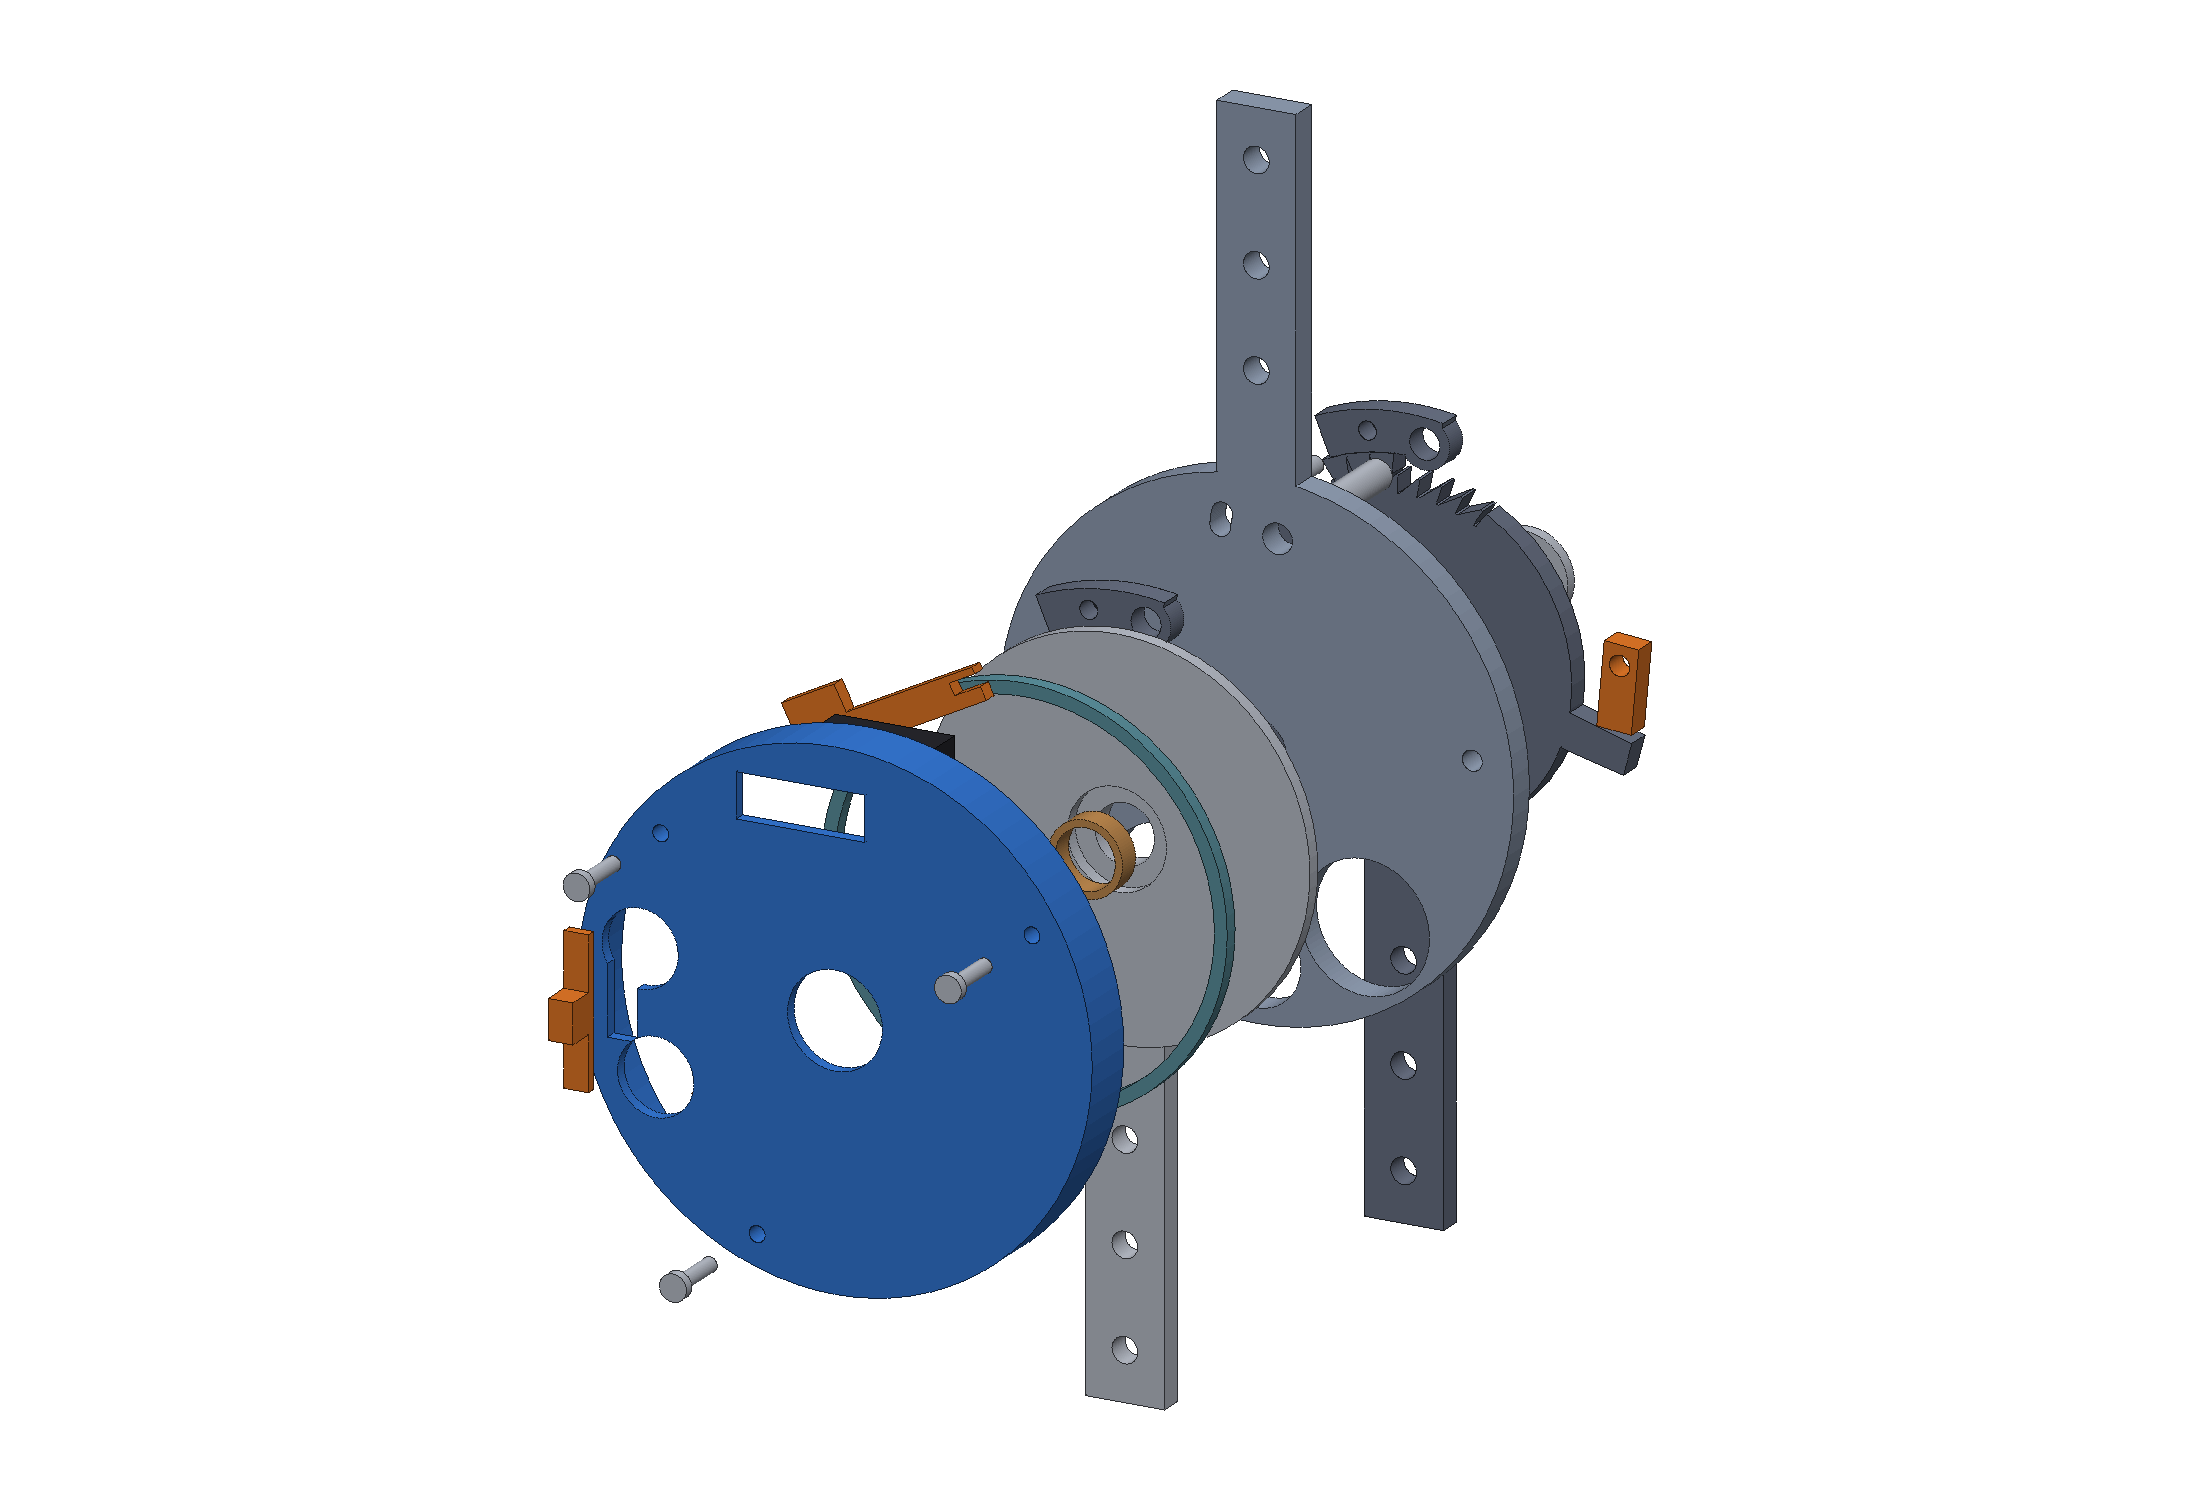
\includegraphics[width=0.50\textwidth]{figures/render_exploded.png}
\caption{\textbf{LATCH joint, lateral side of a right KAFO.} Left: assembled, 104\,mm hub diameter, 26\,mm lateral build; the printed cover carries the three-position mode selector (LOCK / AUTO / FREE), two rotary dampers and the timer dashpot. Right: exploded along the knee axis; from the medial side: toothed inner shank plate with stop lug, inner pawl, thigh plate, toothed outer shank plate (teeth phased half a pitch), outer pawl, direction ring, lift yoke, latch lever, dampers, cover.}
\label{fig:cad}\end{figure}

\begin{figure}[H]\centering
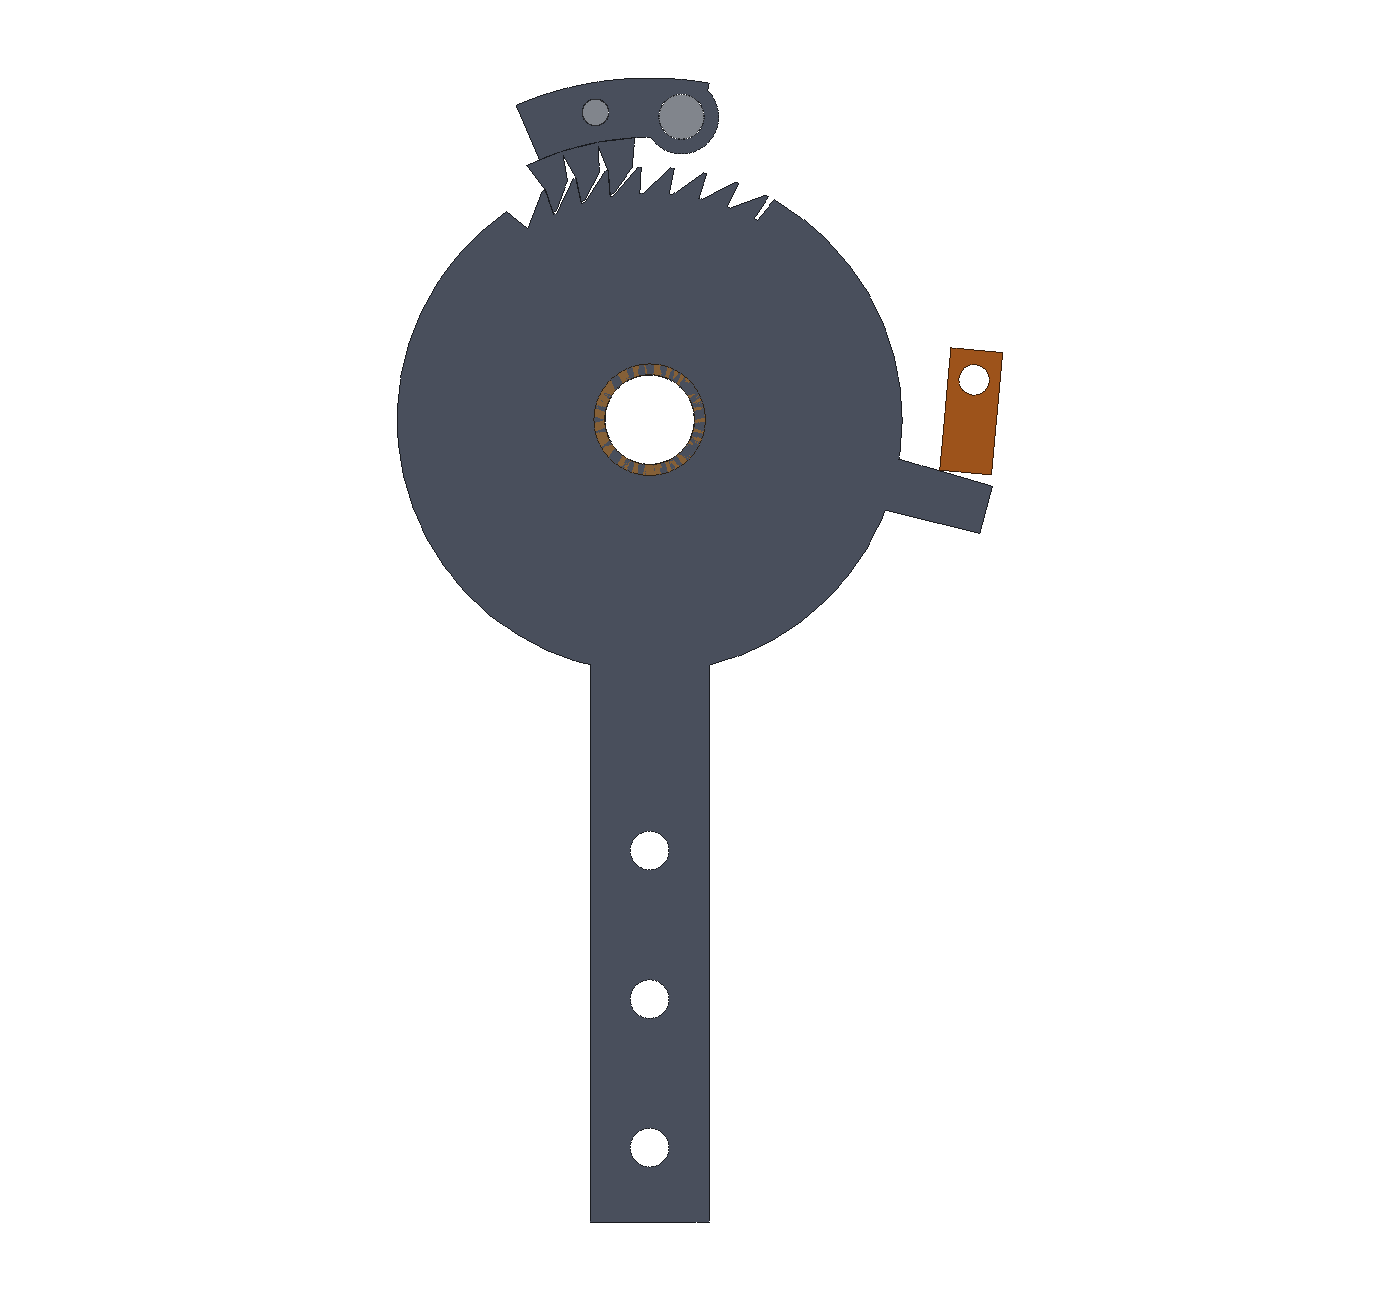
\includegraphics[width=0.32\textwidth]{figures/render_layer_inner_locked.png}\hfill
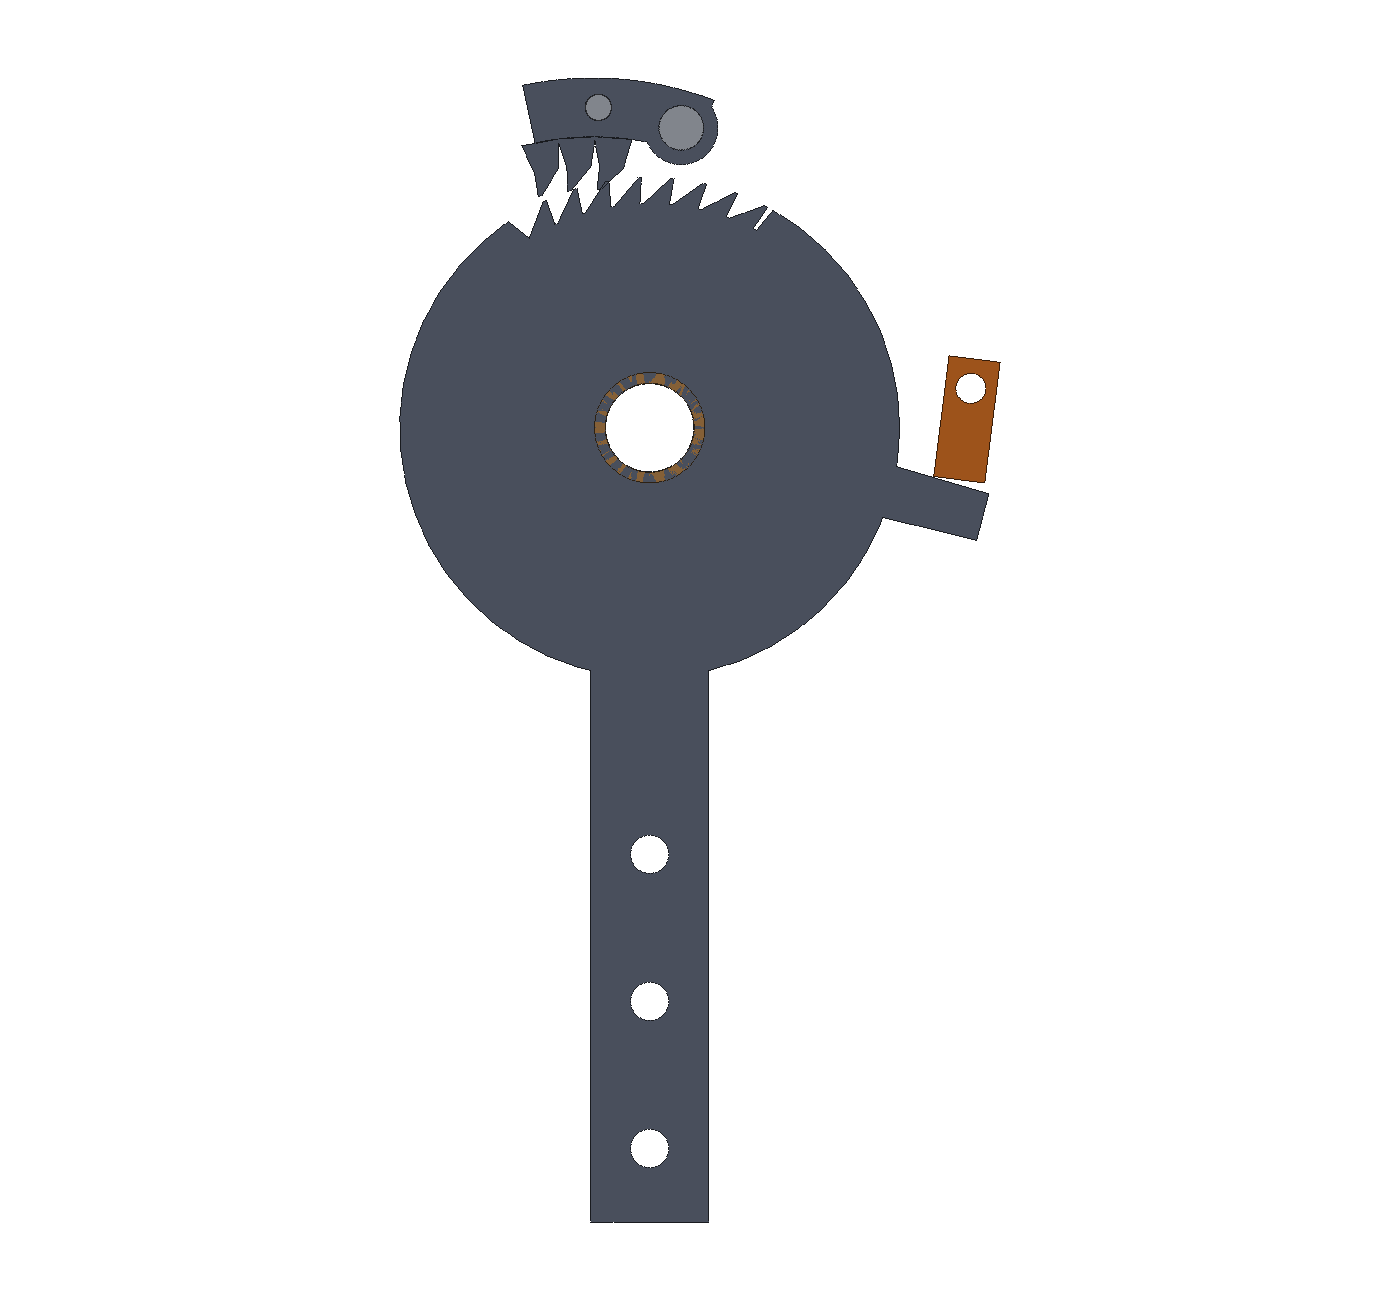
\includegraphics[width=0.32\textwidth]{figures/render_layer_inner_released.png}\hfill
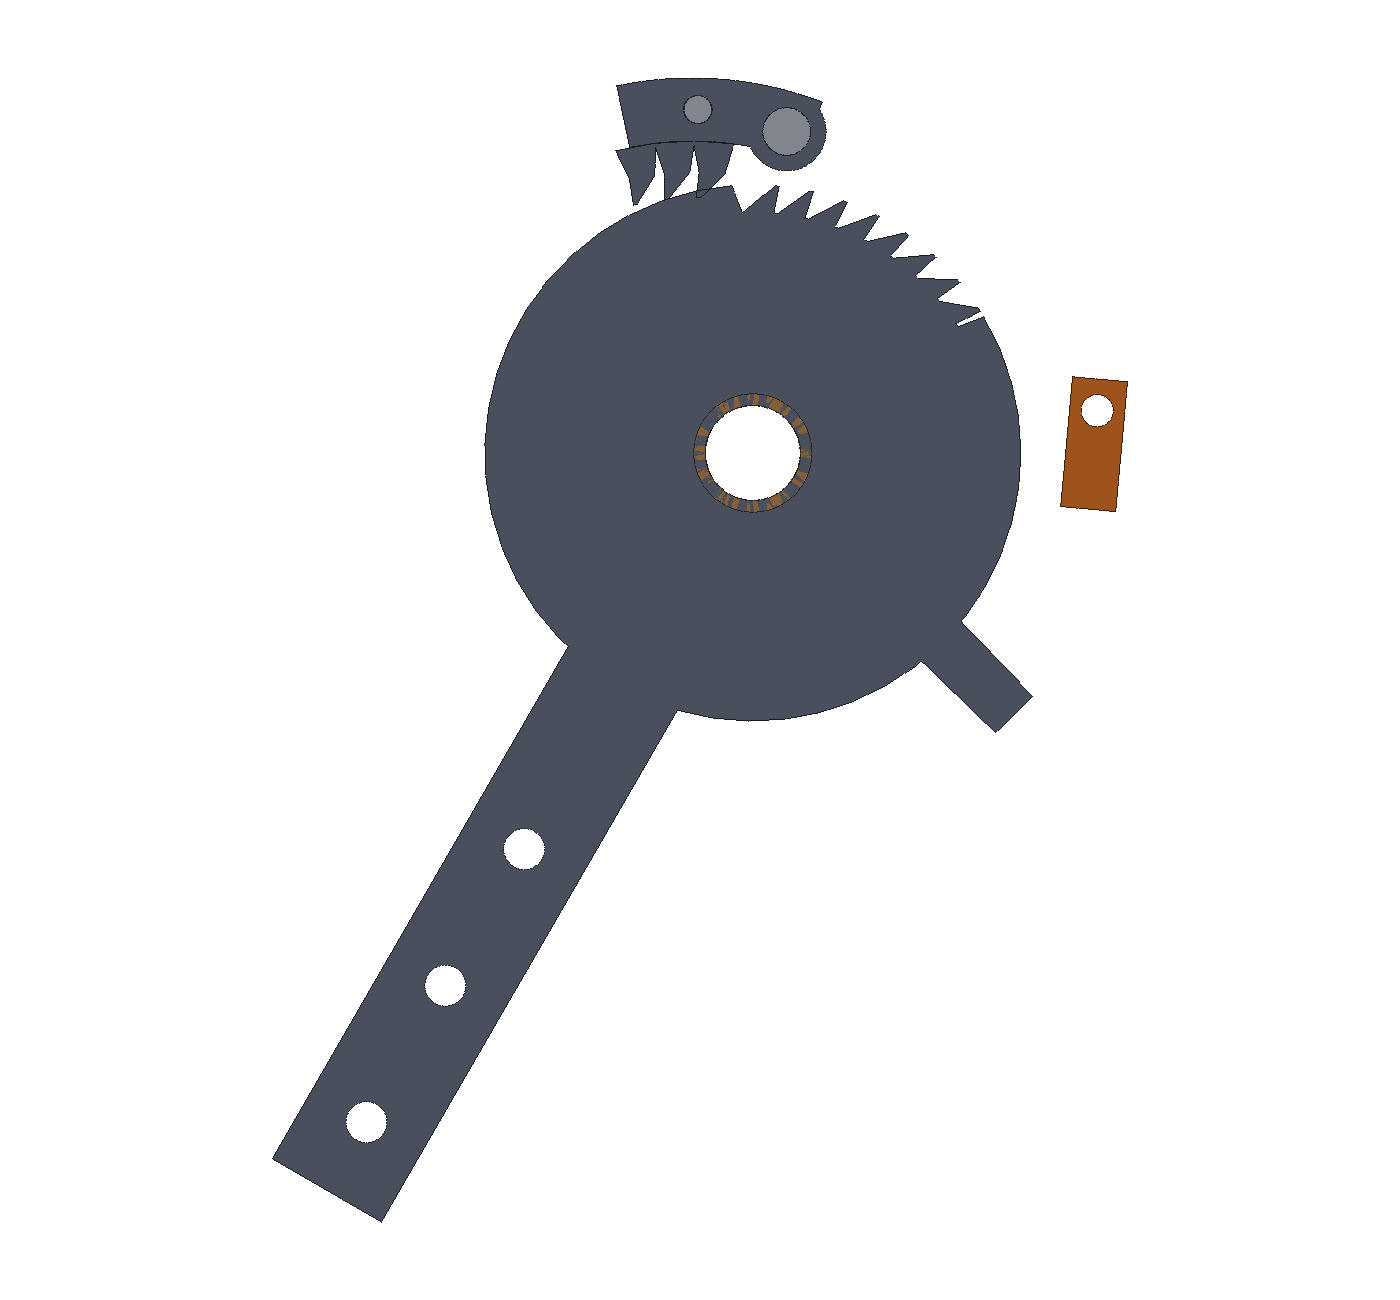
\includegraphics[width=0.32\textwidth]{figures/render_layer_inner_k30.png}
\caption{\textbf{Inner load-path layer} (thigh plate and lateral layers hidden; anterior to the right, proximal up). Left: locked at 0$^\circ$, the three pawl serrations seated against the undercut tooth flanks; the stop lug (anterior) sits 5$^\circ$ from the sprung stop lever (orange). Centre: released, pawl rotated 11$^\circ$ about its pivot, serrations clear of the tooth tips. Right: knee at 30$^\circ$ flexion, the sector has rotated clockwise and the pawl rides the smooth rim at tooth-tip radius.}
\label{fig:layers}\end{figure}

\subsection{Load path}
The joint attaches to standard 16\,mm KAFO uprights. The shank side is a clevis of two 5\,mm laser-cut steel plates whose hubs (34\,mm tip radius) each carry eight ratchet teeth of 7.5$^\circ$ pitch and 3.5\,mm depth over knee angles $-5^\circ$ to $+30^\circ$; the outer plate's teeth are phased by half a pitch, so that with one pawl per plate the knee locks at 3.75$^\circ$ intervals while every tooth has the full 7.5$^\circ$ root. The remaining rim is at tooth-tip radius, so a pawl dropped at large flexion rides onto the teeth without a step. The 6\,mm thigh plate sits between the clevis plates on a 12\,mm shoulder bolt in two flanged bronze bushings. Each pawl is a 5\,mm hook with three serrations that match the tooth spaces; its 6\,mm pivot pin passes through the thigh plate so that both pawls share one pin and are linked by a 3.5\,mm bridge pin through an arc slot in the thigh plate, which the lift yoke drives. The pivot lies about 10$^\circ$ inside the line of action of the tooth force, and the flanks are undercut by 0.6$^\circ$, so the lock is self-energising: load pulls the pawl into the teeth and the pawls can only be lifted when the flexion load is zero, which is the self-holding behaviour assumed in the simulation. Hyperextension is taken by a lug on the inner shank plate against the stop lever on the thigh plate: a die spring preloaded to $M_\mathrm{thr}$ allows 1\,mm of lever travel to actuate the release and then a hard stop carries the remainder of the moment metal-to-metal.

\subsection{Control deck (printed)}
Above the outer plate a 3\,mm deck carries the printed lift yoke (pivoting on the thigh plate, forked over the pawl bridge pin), the spring-steel direction ring (a split friction ring clamped on the outer plate boss whose tab moves 15$^\circ$ between two faces of the yoke arm), the printed latch lever (pushed to ``set'' by the sprung pawl-pin seat when the pawls carry more than $M_\mathrm{pawl}$, returned through a 15\,mm rotary damper giving $T_\mathrm{latch}$), the stop-lever push-rod with its dashpot ($T_\mathrm{long}$) and the second rotary damper on the yoke axis ($t_\mathrm{drop}$). The cover carries a three-position selector: LOCK forces the yoke down and blocks the release path (standing, stairs down), FREE holds the yoke up (sitting, cycling), AUTO is the stance-control mode. The whole deck and cover are PA12-CF prints (about 45\,g); they transmit only spring and damper forces of a few newtons, which is why printed parts are acceptable here and not in the load path.

\subsection{Mass and cost}
The assembly as modelled has 22 components and a computed mass of 963\,g, of which 920\,g is steel; the thigh plate and two shank plates are modelled as full discs and can be pocketed to roughly halve that. The bill of materials (\texttt{latch\_knee\_bom.csv}, 23 lines) totals US\$74 at single-unit prices, dominated by laser-cutting of five steel parts (US\$44) and the three dampers (US\$10), against US\$1{,}700--3{,}500 for commercial mechanical joints \cite{price_freewalk_kit,price_spl2_uk}.

\section{Structural analysis}\label{sec:structural}
Design loads follow from Section~\ref{sec:logic} and the literature: a typical peak external flexion moment of 0.5\,N$\cdot$m/kg (36\,N$\cdot$m for 70\,kg) for fatigue, the 99th-percentile 1.0\,N$\cdot$m/kg (70\,N$\cdot$m) as design moment, and 150\,N$\cdot$m as proof moment, the latter matching the Ottawa piston joint that was designed for $>150$\,N$\cdot$m and survived 400{,}000 cycles \cite{lemaire2009}. Plane-stress finite elements of the toothed plate (Fig.~\ref{fig:fea}) give a von Mises stress at the loaded tooth roots of 250--280\,MPa (99th--99.5th percentile of element stresses) at 70\,N$\cdot$m and 540--600\,MPa at 150\,N$\cdot$m, with a sharp-corner singular maximum of 570 and 1{,}215\,MPa respectively that a 0.4\,mm root fillet removes. For 17-4PH H900 (yield 1{,}170\,MPa, fully reversed fatigue limit about 550\,MPa) or through-hardened 1095 this gives a yield safety factor of 2.0 at the proof moment and a fatigue safety factor above 3 at the typical load (root stress about 140\,MPa). The analytical checks are: tooth tangential force 2{,}170\,N at 70\,N$\cdot$m; 6\,mm pawl pin in double shear 38\,MPa, bearing in the 6\,mm thigh plate 60\,MPa (129\,MPa at proof); 12\,mm knee pin resultant 3.1\,kN, bronze bushing bearing 52\,MPa per plate (93\,MPa at proof); 16$\times$6\,mm thigh upright in sagittal bending 273\,MPa if one upright carries the full 70\,N$\cdot$m (137\,MPa when shared). The FE result also explains why the load path cannot be printed: FFF polyamide-12 and polycarbonate have fatigue limits of 7.4 and 3.6\,MPa \cite{nylon12_pc_fatigue2026} and even short-carbon-fibre polyamide reaches only 40--117\,MPa in tension \cite{scf_pa_fff2021}, two orders of magnitude below the tooth-root stress.

\begin{figure}[H]\centering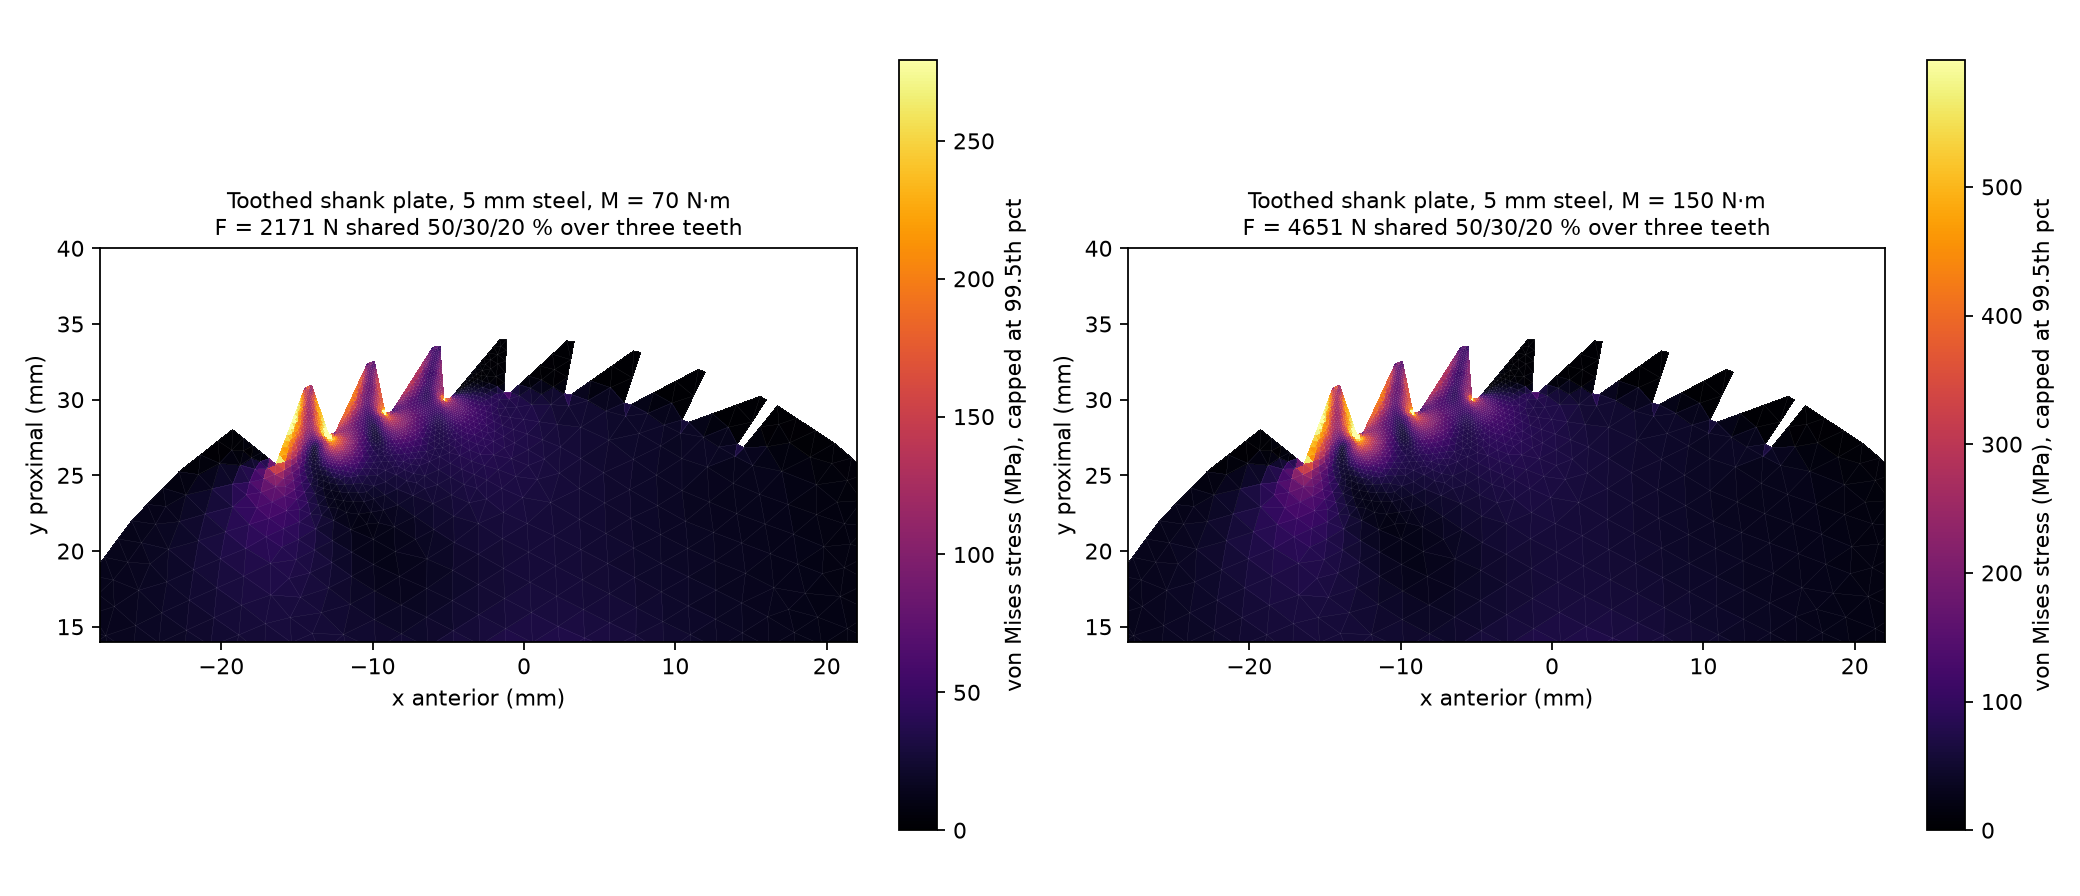
\includegraphics[width=\textwidth]{figures/fig_fea_vm.png}
\caption{\textbf{Plane-stress FE of the toothed shank plate} at the 70\,N$\cdot$m design moment (left) and 150\,N$\cdot$m proof moment (right); 6{,}348 quadratic triangles, fixed at the bushing seat, the tangential tooth force shared 50/30/20\% over the three engaged flanks.}
\label{fig:fea}\end{figure}

\section{Discussion}
\subsection{What the simulation does and does not show}
The simulation is a kinematic/kinetic replay: real knee angles and inverse-dynamics moments of unimpaired walkers drive a causal model of the mechanism, with the knee angle clamped while the lock is engaged. It therefore tests the \emph{decision logic} against the full variability of 51 people at eight speeds, which no bench test can do, but it does not model how a KAFO user's hip and trunk would adapt to the joint, nor the compliance of the orthosis shells, nor friction and wear. Three systematic differences from a KAFO user should bias the results in a known direction. Quadriceps-weak users keep the ground reaction in front of the knee by trunk lean and hyperextension, so their stance moment is extension-dominated: the latch path fires less often and the timer path more often, which the slow-speed rows of Table~\ref{tab:perf} already represent. Their swing is slower and lower, which lengthens the pre-swing window and favours release in time. Their knee hits the extension stop at terminal swing, which the impulse test covers. The one chain that limits fast-walking performance (pre-swing flexion load keeping LATCH live into terminal swing) is specific to vigorous push-off and is unlikely in the target population, but the heel-strike gate that removes it is a cheap addition (an inertia latch on the shank).

\subsection{Comparison with existing joints}
Relative to the pendulum SPL2 the design removes the inertial sensing whose failure we quantified, and relative to the cable-released FreeWalk/UTX family it removes the ankle linkage, so it can be fitted to any KAFO including those with a rigid ankle. Relative to the solenoid joint of Wood and Farris \cite{embc2025solenoid} and the microprocessor joints it needs no battery. Its 3.75$^\circ$ lock resolution is finer than the 10$^\circ$ ratchet of the RESNA prototype \cite{resna2019_eveleight} and comparable to the 2$^\circ$ engagement of the Ottawa piston \cite{lemaire2009}. The release instant (median 28\% of the cycle) is earlier than the heel-off release of cable joints; it is biomechanically justified because the external moment is extension from that instant, but it means the user relies on the extension stop rather than the pawls for the second half of stance, exactly as with every other stance-control joint. The 0.27\% exposure figure is the fraction of strides in which a flexion load appeared while the pawls were up; in all of these the pawls were already dropping (100\,ms delay) and the uncaught flexion in the donor data never exceeded 13$^\circ$.

\subsection{Limitations and next steps}
The CAD is a detailed concept: springs, dampers and the dashpot are modelled as envelopes with specified characteristics, the plates are un-pocketed, and the 963\,g mass must be reduced. The FE is two-dimensional and omits the pawl (sized analytically) and contact; a 3D contact model with a root fillet is the next analysis step. The validation protocol is: (1) static proof test to 150\,N$\cdot$m and ultimate test to failure on an ISO~10328-style rig \cite{iso10328_amd2013}, with strain gauges on the pawl and stop lever to calibrate the two preloads; (2) 400{,}000-cycle fatigue test at 36\,N$\cdot$m with lock--release cycling; (3) bench replay of the WBDS strides on a two-link knee simulator with a programmable moment actuator, which reproduces the exact inputs of this report; (4) gait-laboratory testing with KAFO users on level ground, ramps and stairs with the selector in AUTO and LOCK, measuring lock timing from joint instrumentation and comparing hip hiking, circumduction and oxygen cost with the users' own locked KAFOs, as in \cite{zissimopoulos2007,davis2010}; (5) field evaluation in an LMIC P\&O service, where laser cutting and FFF printing are available and the US\$74 parts cost matters most.

\section{Conclusion}
A knee joint can tell stance from swing from the loads it carries. Driven by 9{,}781 measured strides, the load-sequence logic locks at heel strike in 99.2\% of strides at the speeds KAFO users walk and leaves the knee unprotected under a flexion load in 0.27\%, without any pendulum, cable, battery or sensor, and it locks at whatever angle the knee reaches rather than at one alignment-dependent notch. The same data show why gravity pendulums at the knee cannot be made reliable. The design package (parametric CAD, FE sizing, bill of materials at US\$74, validation protocol) is released so that the next step, a physical prototype on a bench and then on users, can start immediately.

\section*{Data and code availability}
Gait data: Fukuchi et al.\ \cite{fukuchi2018}, figshare 10.6084/m9.figshare.5722711. All analysis code is supplied: \texttt{gait\_pipeline.py} (event detection and kinematics), \texttt{sim\_trigger.py} (pendulum model), \texttt{sim\_lock.py} (load-sequence state machine), \texttt{cad\_knee.py} (parametric CAD, STEP/STL export), \texttt{fea\_ratchet.py} (plane-stress FE), \texttt{make\_figures.py}; result tables \texttt{strides\_design.csv}, \texttt{sweep1.csv}, \texttt{sweep\_seq.csv}, \texttt{lock\_results.json}, \texttt{lock\_sensitivity.json}, \texttt{fea\_results.json}; CAD \texttt{latch\_knee\_assembly.step}, \texttt{latch\_knee\_stl\_parts.zip}; literature base \texttt{references.csv} (137 verified entries) and \texttt{evidence\_summary.md}.

\bibliographystyle{unsrtnat}
\begin{thebibliography}{40}\small
\bibitem{gonzalez2010} Gonzalez H, Olsson T, Borg K. Management of postpolio syndrome. \emph{Lancet Neurol} 2010. doi:10.1016/s1474-4422(10)70095-8
\bibitem{groce2014} Groce NE, Banks LM, Stein MA. Surviving polio in a post-polio world. \emph{Soc Sci Med} 2014. doi:10.1016/j.socscimed.2014.02.024
\bibitem{gbdsci2023} Safdarian M, Trinka E, Rahimi-Movaghar V, et al. Global, regional, and national burden of spinal cord injury, 1990--2019. \emph{Lancet Neurol} 2023. doi:10.1016/S1474-4422(23)00287-9
\bibitem{cooper2012} Cooper A, Alghamdi GA, Alghamdi MA, et al. The relationship of lower limb muscle strength and knee joint hyperextension during the stance phase of gait in hemiparetic stroke patients. \emph{Physiother Res Int} 2011. doi:10.1002/pri.528
\bibitem{locked_kafo_iatrogenic2023} Ghoseiri K, Zucker-Levin A. Long-term locked knee ankle foot orthosis use: a perspective overview of iatrogenic biomechanical and physiological perils. \emph{Front Rehabil Sci} 2023. doi:10.3389/fresc.2023.1138792
\bibitem{yakimovich2009} Yakimovich T, Lemaire ED, Kofman J. Engineering design review of stance-control knee-ankle-foot orthoses. \emph{J Rehabil Res Dev} 2009. doi:10.1682/JRRD.2008.02.0024
\bibitem{phillips1993} Phillips B, Zhao H. Predictors of assistive technology abandonment. \emph{Assist Technol} 1993. doi:10.1080/10400435.1993.10132205
\bibitem{jrm2021_kafo_polio} Raijmakers B, Berendsen-de Gooijer H, Ploeger H, et al. Use and usability of custom-made knee-ankle-foot orthoses in polio survivors. \emph{J Rehabil Med} 2022. doi:10.2340/jrm.v53.1122
\bibitem{who_ispo2017} World Health Organization, ISPO, USAID. \emph{WHO standards for prosthetics and orthotics}. Geneva: WHO; 2017.
\bibitem{ispo_pando_day} International Society for Prosthetics and Orthotics. International Prosthetics and Orthotics Day fact page. ispoint.org, accessed 2026-10-03.
\bibitem{magnusson2017} Magnusson L, Ahlstr\"om G. Patients' satisfaction with lower-limb prosthetic and orthotic devices and service delivery in Sierra Leone and Malawi. \emph{BMC Health Serv Res} 2017. doi:10.1186/s12913-017-2044-3
\bibitem{davis2010} Davis PC, Bach TM, Pereira DM. The effect of stance control orthoses on gait characteristics and energy expenditure in knee-ankle-foot orthosis users. \emph{Prosthet Orthot Int} 2010. doi:10.3109/03093641003773189
\bibitem{zissimopoulos2007} Zissimopoulos A, Fatone S, Gard SA. Biomechanical and energetic effects of a stance-control orthotic knee joint. \emph{J Rehabil Res Dev} 2007. doi:10.1682/jrrd.2006.09.0124
\bibitem{irby2005} Irby SE, Bernhardt KA, Kaufman KR. Gait of stance control orthosis users. \emph{Prosthet Orthot Int} 2005. doi:10.1080/03093640500238915
\bibitem{spl2_manual} Fillauer / Basko. \emph{SPL2 Product Manual}. 2020.
\bibitem{neurotronic2023} Raijmakers B, Brehm MA, Nollet F, et al. Safety, walking ability, and satisfaction outcomes of the NEURO TRONIC stance-control knee joint. \emph{Prosthet Orthot Int} 2023. doi:10.1097/pxr.0000000000000311
\bibitem{schmalz2016} Schmalz T, Pr\"obsting E, Auberger R, Siewert G. A functional comparison of conventional knee-ankle-foot orthoses and a microprocessor-controlled leg orthosis system. \emph{Prosthet Orthot Int} 2016. doi:10.1177/0309364614546524
\bibitem{price_cbrace_sps} SPS / Hanger Fabrication Network. C-Brace process flow, cost and reimbursement (PDF). 2022.
\bibitem{price_freewalk_kit} Ottobock 170K1 FreeWalk kit, US retail listing, accessed 2026-10-03.
\bibitem{price_spl2_uk} De Novo Healthcare (UK). SPL 2 knee joint system (Basko) retail listing, accessed 2026-10-03.
\bibitem{resna2019_eveleight} Eveleigh et al. Design and analysis of a stance-control knee-ankle-foot orthosis. \emph{RESNA 2019 Annual Conference}.
\bibitem{becker_safetystride} Becker Orthopedic. Stride family stance-control knee joints, product pages, accessed 2026-10-03.
\bibitem{yakimovich2006} Yakimovich T, Kofman J, Lemaire ED. Design and evaluation of a stance-control knee-ankle-foot orthosis knee joint. \emph{IEEE Trans Neural Syst Rehabil Eng} 2006. doi:10.1109/tnsre.2006.881578
\bibitem{lemaire2009} Lemaire ED, Samadi R, Goudreau L, Kofman J. Mechanical and biomechanical analysis of a linear piston design for angular-velocity-based orthotic control. \emph{J Rehabil Res Dev} 2013. doi:10.1682/jrrd.2012.02.0031
\bibitem{shamaei2014} Shamaei K, Napolitano PC, Dollar AM. Design and functional evaluation of a quasi-passive compliant stance control knee-ankle-foot orthosis. \emph{IEEE Trans Neural Syst Rehabil Eng} 2014. doi:10.1109/tnsre.2014.2305664
\bibitem{embc2025solenoid} Wood, Farris. Design of a low-cost solenoid actuated stance control knee orthosis. \emph{Proc IEEE EMBC} 2025. doi:10.1109/embc58623.2025.11254937
\bibitem{fukuchi2018} Fukuchi CA, Fukuchi RK, Duarte M. A public dataset of overground and treadmill walking kinematics and kinetics in healthy individuals. \emph{PeerJ} 2018. doi:10.7717/peerj.4640
\bibitem{nylon12_pc_fatigue2026} Rodrigues, Branco, Franco, et al. Mechanical, fatigue, and thermal characterization of ASA, Nylon 12, PC and PC-ABS produced by FFF. \emph{Polymers} 2026. doi:10.3390/polym18020302
\bibitem{scf_pa_fff2021} Abderrafai Y, Hadi Mahdavi M, Sosa-Rey F, et al. Additive manufacturing of short carbon fiber-reinforced polyamide composites by fused filament fabrication. \emph{Mater Des} 2022. doi:10.1016/j.matdes.2021.110358
\bibitem{iso10328_amd2013} ISO 10328:2006/Amd 1:2013. Prosthetics -- Structural testing of lower-limb prostheses -- Requirements and test methods. Geneva: ISO.
\end{thebibliography}
\end{document}
